\documentclass[aspectratio=169]{beamer}
\usetheme{Madrid}
\usecolortheme{default}

\usepackage{amsmath, amsfonts}
\usepackage{booktabs}
\usepackage{tikz}
\usetikzlibrary{arrows.meta, calc}
\usepackage{pgfplots}
\usepgfplotslibrary{groupplots}
\pgfplotsset{compat=1.18}
\usepackage{listings}
\usepackage{xcolor}

\lstset{
    basicstyle=\ttfamily\tiny,
    keywordstyle=\color{blue}\bfseries,
    commentstyle=\color{green!60!black},
    stringstyle=\color{red},
    breaklines=true,
    frame=single,
    backgroundcolor=\color{gray!10},
    language=Python,
    showstringspaces=false,
    aboveskip=2pt,
    belowskip=2pt
}

\title{GAMs in Practice}
\subtitle{Distributions, link functions, and functional forms with pyGAM}
\author{CSE255 - Scalable Data Analysis}
\date{\today}

\begin{document}

\frame{\titlepage}

% --- Slide 2: Construction figure (visual recursion) ---
\begin{frame}{Cox--de Boor construction (visual)}
\small
\textbf{Raise the degree by blending neighbors.} At each step, a level-$(d+1)$ function is built from \emph{two} level-$d$ functions with $x$-dependent weights.

\vspace{1mm}
\centering
\begin{tabular}{c@{\hspace{4mm}}c@{\hspace{4mm}}c}
\begin{minipage}{0.42\textwidth}\centering
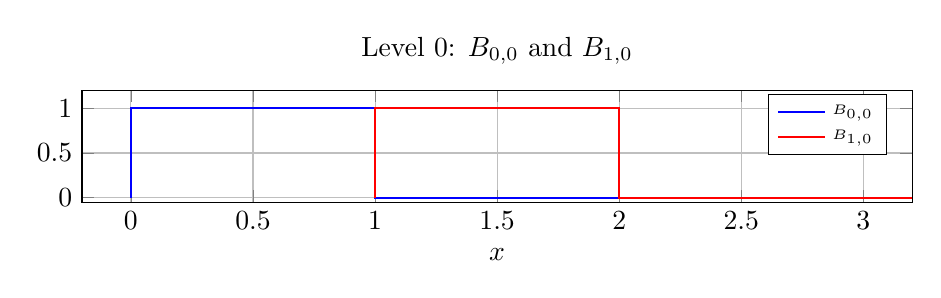
\begin{tikzpicture}
\begin{axis}[width=\linewidth, height=3.0cm,
  title={Level 0: $B_{0,0}$ and $B_{1,0}$},
  xlabel={$x$}, ylabel={}, grid=major,
  xmin=-0.2, xmax=3.2, ymin=-0.05, ymax=1.2,
  legend pos=north east, legend style={font=\tiny}]
\addplot[thick, blue] coordinates {(0,0)(0,1)(1,1)(1,0)(3.2,0)};
\addplot[thick, red]  coordinates {(1,0)(1,1)(2,1)(2,0)(3.2,0)};
\legend{$B_{0,0}$, $B_{1,0}$}
\end{axis}
\end{tikzpicture}
\end{minipage}
&
\begin{minipage}{0.06\textwidth}\centering
\(\Rightarrow\)
\end{minipage}
&
\begin{minipage}{0.42\textwidth}\centering
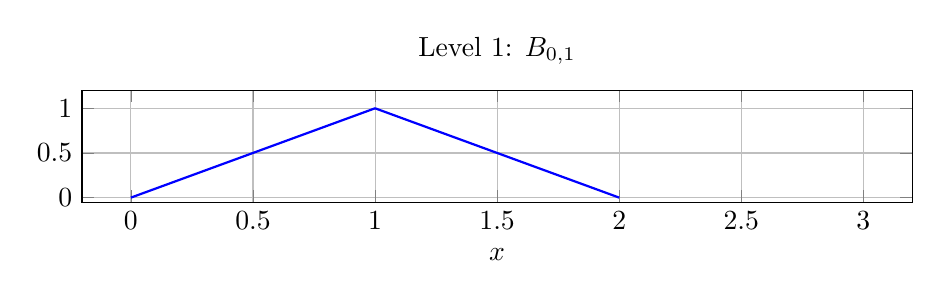
\begin{tikzpicture}
\begin{axis}[width=\linewidth, height=3.0cm,
  title={Level 1: $B_{0,1}$},
  xlabel={$x$}, ylabel={}, grid=major,
  xmin=-0.2, xmax=3.2, ymin=-0.05, ymax=1.2]
\addplot[thick, blue, domain=0:1, samples=40] {x};
\addplot[thick, blue, domain=1:2, samples=40] {2-x};
\end{axis}
\end{tikzpicture}
\end{minipage}
\\[0.8mm]
\begin{minipage}{0.42\textwidth}\centering
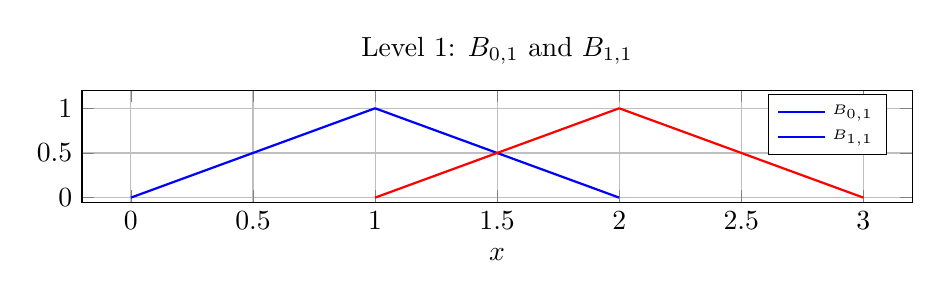
\begin{tikzpicture}
\begin{axis}[width=\linewidth, height=3.0cm,
  title={Level 1: $B_{0,1}$ and $B_{1,1}$},
  xlabel={$x$}, ylabel={}, grid=major,
  xmin=-0.2, xmax=3.2, ymin=-0.05, ymax=1.2,
  legend pos=north east, legend style={font=\tiny}]
\addplot[thick, blue, domain=0:1, samples=40] {x};
\addplot[thick, blue, domain=1:2, samples=40] {2-x};
\addplot[thick, red,  domain=1:2, samples=40] {x-1};
\addplot[thick, red,  domain=2:3, samples=40] {3-x};
\legend{$B_{0,1}$, $B_{1,1}$}
\end{axis}
\end{tikzpicture}
\end{minipage}
&
\begin{minipage}{0.06\textwidth}\centering
\(\Rightarrow\)
\end{minipage}
&
\begin{minipage}{0.42\textwidth}\centering
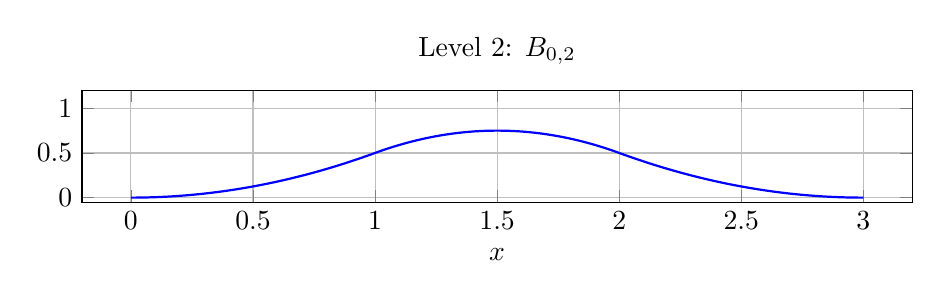
\begin{tikzpicture}
\begin{axis}[width=\linewidth, height=3.0cm,
  title={Level 2: $B_{0,2}$},
  xlabel={$x$}, ylabel={}, grid=major,
  xmin=-0.2, xmax=3.2, ymin=-0.05, ymax=1.2]
\addplot[thick, blue, domain=0:1, samples=60] {0.5*x*x};
\addplot[thick, blue, domain=1:2, samples=60] {3*x - x*x - 1.5};
\addplot[thick, blue, domain=2:3, samples=60] {0.5*(3-x)*(3-x)};
\end{axis}
\end{tikzpicture}
\end{minipage}
\end{tabular}

\vspace{0mm}\scriptsize Degree-raising widens support by one knot interval and increases smoothness.
\end{frame}

% --- Slide 3: Formulas (annotated) ---
\begin{frame}{Cox--de Boor recursion (annotated)}
\small
Choose knots $t_0 \le \cdots \le t_m$. Define basis functions by degree:
\[
B_{j,0}(x) =
\begin{cases}
1 & t_j \le x < t_{j+1}\\
0 & \text{otherwise}
\end{cases}
\qquad
\text{(piecewise constant)}
\]
\vspace{-1mm}
\[
B_{j,d}(x) =
\underbrace{\frac{x - t_j}{t_{j+d} - t_j}}_{\text{ramps up on }[t_j,t_{j+d}]}\, B_{j,d-1}(x)
\;+\;
\underbrace{\frac{t_{j+d+1} - x}{t_{j+d+1} - t_{j+1}}}_{\text{ramps down on }[t_{j+1},t_{j+d+1}]}\, B_{j+1,d-1}(x)
\]
\begin{itemize}
    \item \textbf{Local support}: $B_{j,d}(x)=0$ outside $[t_j,\,t_{j+d+1}]$ (only $d+1$ knot intervals).
    \item \textbf{Nonnegative + partition of unity}: $B_{j,d}(x)\ge 0$ and the overlapping bumps sum to 1 inside the knot range.
    \item \textbf{Smoothness}: degree $d$ gives $C^{d-1}$ continuity at interior knots (e.g.\ cubic $\Rightarrow C^2$).
\end{itemize}
\end{frame}

% --- Slide 4: Basis functions for degrees 0..3 (robust layout) ---
\begin{frame}{Basis functions by degree (0--3)}
\centering
\small Uniform knots $t_i=i$ for $i=0,\ldots,7$.
\vspace{1mm}
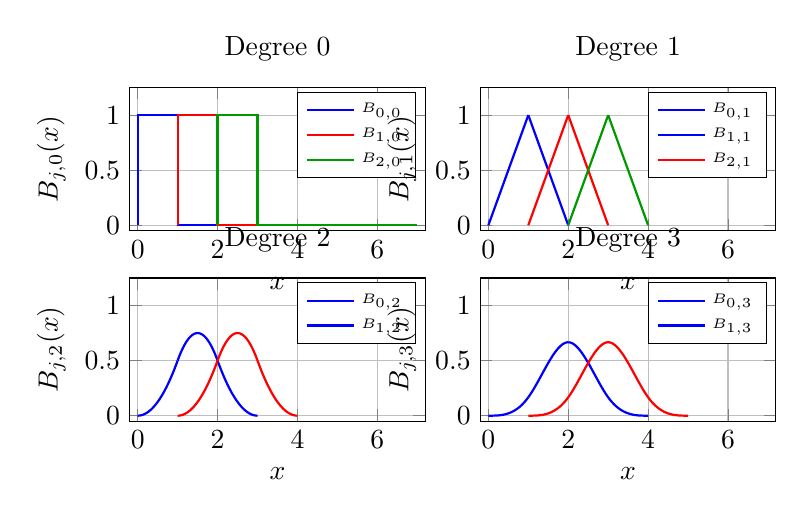
\begin{tikzpicture}
\begin{groupplot}[
  group style={group size=2 by 2, horizontal sep=7mm, vertical sep=6mm},
  width=0.44\textwidth, height=3.4cm,
  grid=major, xmin=-0.2, xmax=7.2, ymin=-0.05, ymax=1.25,
  legend style={font=\tiny},
]
\nextgroupplot[title={Degree 0}, xlabel={$x$}, ylabel={$B_{j,0}(x)$}, legend pos=north east]
\addplot[thick, blue] coordinates {(0,0)(0,1)(1,1)(1,0)(7,0)};
\addplot[thick, red]  coordinates {(1,0)(1,1)(2,1)(2,0)(7,0)};
\addplot[thick, green!60!black] coordinates {(2,0)(2,1)(3,1)(3,0)(7,0)};
\legend{$B_{0,0}$, $B_{1,0}$, $B_{2,0}$}

\nextgroupplot[title={Degree 1}, xlabel={$x$}, ylabel={$B_{j,1}(x)$}, legend pos=north east]
\addplot[thick, blue, domain=0:1, samples=30] {x};
\addplot[thick, blue, domain=1:2, samples=30] {2-x};
\addplot[thick, red,  domain=1:2, samples=30] {x-1};
\addplot[thick, red,  domain=2:3, samples=30] {3-x};
\addplot[thick, green!60!black, domain=2:3, samples=30] {x-2};
\addplot[thick, green!60!black, domain=3:4, samples=30] {4-x};
\legend{$B_{0,1}$, $B_{1,1}$, $B_{2,1}$}

\nextgroupplot[title={Degree 2}, xlabel={$x$}, ylabel={$B_{j,2}(x)$}, legend pos=north east]
\addplot[thick, blue, domain=0:1, samples=40] {0.5*x*x};
\addplot[thick, blue, domain=1:2, samples=40] {3*x - x*x - 1.5};
\addplot[thick, blue, domain=2:3, samples=40] {0.5*(3-x)*(3-x)};
\addplot[thick, red,  domain=1:2, samples=40] {0.5*(x-1)*(x-1)};
\addplot[thick, red,  domain=2:3, samples=40] {-(x-2)*(x-2) + (x-2) + 0.5};
\addplot[thick, red,  domain=3:4, samples=40] {0.5*(4-x)*(4-x)};
\legend{$B_{0,2}$, $B_{1,2}$}

\nextgroupplot[title={Degree 3}, xlabel={$x$}, ylabel={$B_{j,3}(x)$}, legend pos=north east]
\addplot[thick, blue, domain=0:1, samples=40] {x*x*x/6};
\addplot[thick, blue, domain=1:2, samples=40] {(-3*(x-1)^3 + 3*(x-1)^2 + 3*(x-1) + 1)/6};
\addplot[thick, blue, domain=2:3, samples=40] {(3*(x-2)^3 - 6*(x-2)^2 + 4)/6};
\addplot[thick, blue, domain=3:4, samples=40] {(4-x)^3/6};
\addplot[thick, red,  domain=1:2, samples=40] {(x-1)^3/6};
\addplot[thick, red,  domain=2:3, samples=40] {(-3*(x-2)^3 + 3*(x-2)^2 + 3*(x-2) + 1)/6};
\addplot[thick, red,  domain=3:4, samples=40] {(3*(x-3)^3 - 6*(x-3)^2 + 4)/6};
\addplot[thick, red,  domain=4:5, samples=40] {(5-x)^3/6};
\legend{$B_{0,3}$, $B_{1,3}$}
\end{groupplot}
\end{tikzpicture}
\end{frame}

% --- Slide 5: Spacing and width given data ---
\begin{frame}{Spacing and width given data $x_1, \ldots, x_n$}
\small
From data $x_1, \ldots, x_n$ we choose a \textbf{knot sequence} (e.g.\ range $[a,b]$ and interior knots), which fixes \textbf{where} the basis functions sit and \textbf{how wide} they are in $x$.

\begin{itemize}
    \item \textbf{Knot placement}: Often knots at \textbf{quantiles} of $\{x_i\}$ (so more knots where data are dense), or \textbf{equally spaced} in $[a,b]$. Endpoints $t_0 = a$, $t_m = b$ (or slightly extended).
    \item \textbf{Number of basis functions}: With $m+1$ knots and degree $d$, $K = m - d$. Choice of $K$ (e.g.\ \texttt{n\_splines} in pyGAM) plus knot rule determines how many bumps and where they sit.
    \item \textbf{Support (width)}: Each $B_{j,d}$ is non-zero on \textbf{$d+1$ consecutive knot intervals}. So ``width in number of intervals'' is the same for all $j$; \textbf{width in $x$} = sum of those interval lengths $\Rightarrow$ same for all $j$ only when knots are \emph{uniform}; with quantile knots, bumps are narrower where data are dense, wider where sparse.
\end{itemize}
\end{frame}

% --- Slide 6: Spacing/width summary and figure ---
\begin{frame}{Spacing and width: uniform vs quantile knots}
\small
\begin{columns}[T]
\begin{column}{0.5\textwidth}
\textbf{Uniform knots} $t_{i+1}-t_i = h$:
\begin{itemize}
    \item Same width in $x$ for every $B_j$: $(d+1)h$.
    \item Bumps evenly spaced; regular overlap.
\end{itemize}
\vspace{2mm}
\textbf{Quantile-based knots} (e.g.\ $K$ interior knots at sample quantiles):
\begin{itemize}
    \item Width in $x$ \emph{varies}: narrow where data dense, wide where sparse.
    \item More basis activity where you have more data.
\end{itemize}
\end{column}
\begin{column}{0.5\textwidth}
\centering
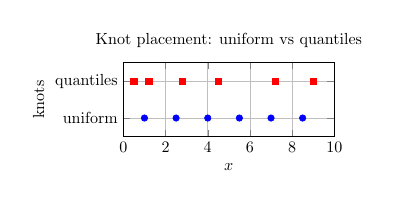
\begin{tikzpicture}[scale=0.58]
\begin{axis}[width=6.2cm, height=3.2cm, xlabel={$x$}, ylabel={knots},
  title={Knot placement: uniform vs quantiles},
  ymin=-0.5, ymax=1.5, ytick={0,1}, yticklabels={uniform, quantiles},
  xmin=0, xmax=10, grid=major]
\addplot[only marks, mark=*, blue] coordinates {(1,0) (2.5,0) (4,0) (5.5,0) (7,0) (8.5,0)};
\addplot[only marks, mark=square*, red] coordinates {(0.5,1) (1.2,1) (2.8,1) (4.5,1) (7.2,1) (9,1)};
\end{axis}
\end{tikzpicture}
\vspace{1mm}
\scriptsize
Top: equal spacing. Bottom: denser knots where data pile up.
\end{column}
\end{columns}
\end{frame}

% --- Non-uniform knots: what changes? ---
\begin{frame}{When knots are not equally spaced: what changes?}
\small
Let $t_0 \le \cdots \le t_m$ be \textbf{non-uniform} (unequal gaps).
\begin{itemize}
    \item \textbf{Support still spans $d+1$ intervals}: $B_{j,d}(x)=0$ outside $[t_j,\,t_{j+d+1}]$.
    \item \textbf{But width in $x$ varies}: the physical width is $\sum_{k=j}^{j+d} (t_{k+1}-t_k)$, which changes with local knot gaps.
    \item \textbf{Shapes become asymmetric}: for $d\ge 1$, the left/right slopes (and where the peak sits relative to the support) depend on the adjacent interval lengths.
    \item \textbf{More resolution where knots are dense}: tight knot spacing gives narrow, local basis functions; wide gaps give broad basis functions.
\end{itemize}
\vspace{1mm}
\textbf{Interpretation:} non-uniform knots adapt the basis to the geometry/density of $x$ (often via quantiles or domain-specific placement).
\end{frame}

% --- Non-uniform knots: exact figure for degree 0 and 1 ---
\begin{frame}{Non-uniform knots: basis functions get uneven widths (example)}
\centering
\small Example knot sequence (non-uniform): $t = (0,\; 1,\; 1.6,\; 3.0,\; 4.7,\; 5.0)$.
\vspace{1mm}
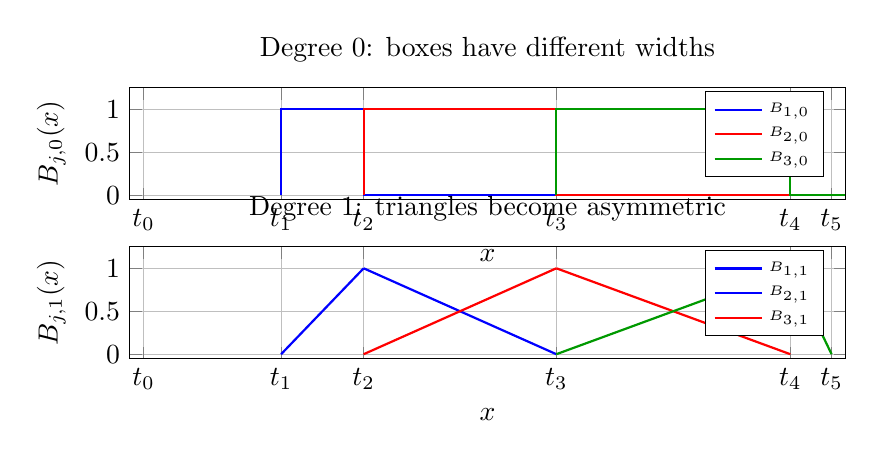
\begin{tikzpicture}
\begin{groupplot}[
  group style={group size=1 by 2, vertical sep=6mm},
  width=0.88\textwidth, height=3.0cm,
  grid=major, xmin=-0.1, xmax=5.1, ymin=-0.05, ymax=1.25,
  xtick={0,1,1.6,3.0,4.7,5.0},
  xticklabels={$t_0$,$t_1$,$t_2$,$t_3$,$t_4$,$t_5$},
]
\nextgroupplot[title={Degree 0: boxes have different widths}, xlabel={$x$}, ylabel={$B_{j,0}(x)$}, legend style={font=\tiny}, legend pos=north east]
% B_{1,0} on [t1,t2] = [1,1.6]
\addplot[thick, blue] coordinates {(1,0)(1,1)(1.6,1)(1.6,0)(5.1,0)};
% B_{2,0} on [t2,t3] = [1.6,3.0]
\addplot[thick, red]  coordinates {(1.6,0)(1.6,1)(3.0,1)(3.0,0)(5.1,0)};
% B_{3,0} on [t3,t4] = [3.0,4.7]
\addplot[thick, green!60!black] coordinates {(3.0,0)(3.0,1)(4.7,1)(4.7,0)(5.1,0)};
\legend{$B_{1,0}$, $B_{2,0}$, $B_{3,0}$}

\nextgroupplot[title={Degree 1: triangles become asymmetric}, xlabel={$x$}, ylabel={$B_{j,1}(x)$}, legend style={font=\tiny}, legend pos=north east]
% B_{1,1} support [t1,t3] = [1,3.0], peak at t2=1.6
\addplot[thick, blue, domain=1:1.6, samples=40] {(x-1)/(1.6-1)};
\addplot[thick, blue, domain=1.6:3.0, samples=40] {(3.0-x)/(3.0-1.6)};
% B_{2,1} support [t2,t4] = [1.6,4.7], peak at t3=3.0
\addplot[thick, red, domain=1.6:3.0, samples=40] {(x-1.6)/(3.0-1.6)};
\addplot[thick, red, domain=3.0:4.7, samples=40] {(4.7-x)/(4.7-3.0)};
% B_{3,1} support [t3,t5] = [3.0,5.0], peak at t4=4.7 (very skewed: short right tail)
\addplot[thick, green!60!black, domain=3.0:4.7, samples=40] {(x-3.0)/(4.7-3.0)};
\addplot[thick, green!60!black, domain=4.7:5.0, samples=40] {(5.0-x)/(5.0-4.7)};
\legend{$B_{1,1}$, $B_{2,1}$, $B_{3,1}$}
\end{groupplot}
\end{tikzpicture}
\vspace{1mm}
\scriptsize Same \emph{number} of intervals in the support (here: 2) does \emph{not} mean the same width in $x$ when knot gaps differ.
\end{frame}

% --- Percentile (decile) knots + cubic basis functions ---
\begin{frame}{Decile percentile knots (non-uniform distribution) and cubic basis}
\small
\textbf{Percentile knots:} place knots at $0\%,10\%,\ldots,100\%$ of a \emph{non-uniform} distribution of $x$.
Because the density is uneven, these percentile points are \textbf{not equally spaced in $x$}, and the cubic B-spline basis functions inherit that uneven width.

% Auto-generated from a non-uniform density on [0,1]
\def\NonUniformDensity{
(0.00000,0.00000) (0.01250,0.00000) (0.02500,0.00010) (0.03750,0.00029) (0.05000,0.00080) (0.06250,0.00212) (0.07500,0.00524) (0.08750,0.01218)
(0.10000,0.02659) (0.11250,0.05456) (0.12500,0.10518) (0.13750,0.19045) (0.15000,0.32397) (0.16250,0.51770) (0.17500,0.77715) (0.18750,1.09596)
(0.20000,1.45191) (0.21250,1.80694) (0.22500,2.11252) (0.23750,2.32015) (0.25000,2.39380) (0.26250,2.32015) (0.27500,2.11253) (0.28750,1.80694)
(0.30000,1.45193) (0.31250,1.09599) (0.32500,0.77721) (0.33750,0.51782) (0.35000,0.32421) (0.36250,0.19093) (0.37500,0.10609) (0.38750,0.05626)
(0.40000,0.02968) (0.41250,0.01765) (0.42500,0.01472) (0.43750,0.01815) (0.45000,0.02725) (0.46250,0.04286) (0.47500,0.06697) (0.48750,0.10255)
(0.50000,0.15339) (0.51250,0.22394) (0.52500,0.31905) (0.53750,0.44361) (0.55000,0.60192) (0.56250,0.79702) (0.57500,1.02991) (0.58750,1.29876)
(0.60000,1.59828) (0.61250,1.91944) (0.62500,2.24954) (0.63750,2.57282) (0.65000,2.87159) (0.66250,3.12775) (0.67500,3.32460) (0.68750,3.44861)
(0.70000,3.49096) (0.71250,3.44861) (0.72500,3.32460) (0.73750,3.12775) (0.75000,2.87159) (0.76250,2.57282) (0.77500,2.24954) (0.78750,1.91944)
(0.80000,1.59828) (0.81250,1.29876) (0.82500,1.02991) (0.83750,0.79702) (0.85000,0.60192) (0.86250,0.44361) (0.87500,0.31905) (0.88750,0.22393)
(0.90000,0.15338) (0.91250,0.10252) (0.92500,0.06688) (0.93750,0.04257) (0.95000,0.02645) (0.96250,0.01603) (0.97500,0.00949) (0.98750,0.00548)
(1.00000,0.00309)
}
\def\CubicBasisA{
(0.00000,0.00000) (0.01250,0.00000) (0.02500,0.00000) (0.03750,0.00000) (0.05000,0.00000) (0.06250,0.00000) (0.07500,0.00000) (0.08750,0.00000)
(0.10000,0.00000) (0.11250,0.00000) (0.12500,0.00000) (0.13750,0.00000) (0.15000,0.00000) (0.16250,0.00000) (0.17500,0.00000) (0.18750,0.00000)
(0.20000,0.00000) (0.21250,0.00000) (0.22500,0.00000) (0.23750,0.00024) (0.25000,0.00322) (0.26250,0.01272) (0.27500,0.03249) (0.28750,0.06424)
(0.30000,0.10598) (0.31250,0.15534) (0.32500,0.20993) (0.33750,0.26740) (0.35000,0.32535) (0.36250,0.38142) (0.37500,0.43323) (0.38750,0.47841)
(0.40000,0.51458) (0.41250,0.53937) (0.42500,0.55074) (0.43750,0.54914) (0.45000,0.53611) (0.46250,0.51315) (0.47500,0.48181) (0.48750,0.44361)
(0.50000,0.40007) (0.51250,0.35273) (0.52500,0.30311) (0.53750,0.25275) (0.55000,0.20316) (0.56250,0.15588) (0.57500,0.11244) (0.58750,0.07436)
(0.60000,0.04316) (0.61250,0.02039) (0.62500,0.00711) (0.63750,0.00138) (0.65000,0.00000) (0.66250,0.00000) (0.67500,0.00000) (0.68750,0.00000)
(0.70000,0.00000) (0.71250,0.00000) (0.72500,0.00000) (0.73750,0.00000) (0.75000,0.00000) (0.76250,0.00000) (0.77500,0.00000) (0.78750,0.00000)
(0.80000,0.00000) (0.81250,0.00000) (0.82500,0.00000) (0.83750,0.00000) (0.85000,0.00000) (0.86250,0.00000) (0.87500,0.00000) (0.88750,0.00000)
(0.90000,0.00000) (0.91250,0.00000) (0.92500,0.00000) (0.93750,0.00000) (0.95000,0.00000) (0.96250,0.00000) (0.97500,0.00000) (0.98750,0.00000)
(1.00000,0.00000)
}
\def\CubicBasisB{
(0.00000,0.00000) (0.01250,0.00000) (0.02500,0.00000) (0.03750,0.00000) (0.05000,0.00000) (0.06250,0.00000) (0.07500,0.00000) (0.08750,0.00000)
(0.10000,0.00000) (0.11250,0.00000) (0.12500,0.00000) (0.13750,0.00000) (0.15000,0.00000) (0.16250,0.00000) (0.17500,0.00000) (0.18750,0.00000)
(0.20000,0.00000) (0.21250,0.00000) (0.22500,0.00000) (0.23750,0.00000) (0.25000,0.00000) (0.26250,0.00000) (0.27500,0.00000) (0.28750,0.00022)
(0.30000,0.00122) (0.31250,0.00365) (0.32500,0.00811) (0.33750,0.01524) (0.35000,0.02564) (0.36250,0.03995) (0.37500,0.05879) (0.38750,0.08277)
(0.40000,0.11253) (0.41250,0.14867) (0.42500,0.19160) (0.43750,0.24004) (0.45000,0.29202) (0.46250,0.34555) (0.47500,0.39862) (0.48750,0.44927)
(0.50000,0.49549) (0.51250,0.53530) (0.52500,0.56671) (0.53750,0.58774) (0.55000,0.59638) (0.56250,0.59066) (0.57500,0.56859) (0.58750,0.52817)
(0.60000,0.46742) (0.61250,0.38435) (0.62500,0.27937) (0.63750,0.16883) (0.65000,0.07557) (0.66250,0.02074) (0.67500,0.00200) (0.68750,0.00000)
(0.70000,0.00000) (0.71250,0.00000) (0.72500,0.00000) (0.73750,0.00000) (0.75000,0.00000) (0.76250,0.00000) (0.77500,0.00000) (0.78750,0.00000)
(0.80000,0.00000) (0.81250,0.00000) (0.82500,0.00000) (0.83750,0.00000) (0.85000,0.00000) (0.86250,0.00000) (0.87500,0.00000) (0.88750,0.00000)
(0.90000,0.00000) (0.91250,0.00000) (0.92500,0.00000) (0.93750,0.00000) (0.95000,0.00000) (0.96250,0.00000) (0.97500,0.00000) (0.98750,0.00000)
(1.00000,0.00000)
}
\def\CubicBasisC{
(0.00000,0.00000) (0.01250,0.00000) (0.02500,0.00000) (0.03750,0.00000) (0.05000,0.00000) (0.06250,0.00000) (0.07500,0.00000) (0.08750,0.00000)
(0.10000,0.00000) (0.11250,0.00000) (0.12500,0.00000) (0.13750,0.00000) (0.15000,0.00000) (0.16250,0.00000) (0.17500,0.00000) (0.18750,0.00000)
(0.20000,0.00000) (0.21250,0.00000) (0.22500,0.00000) (0.23750,0.00000) (0.25000,0.00000) (0.26250,0.00000) (0.27500,0.00000) (0.28750,0.00000)
(0.30000,0.00000) (0.31250,0.00000) (0.32500,0.00000) (0.33750,0.00000) (0.35000,0.00000) (0.36250,0.00000) (0.37500,0.00000) (0.38750,0.00000)
(0.40000,0.00000) (0.41250,0.00000) (0.42500,0.00008) (0.43750,0.00089) (0.45000,0.00334) (0.46250,0.00833) (0.47500,0.01676) (0.48750,0.02954)
(0.50000,0.04757) (0.51250,0.07176) (0.52500,0.10300) (0.53750,0.14220) (0.55000,0.19028) (0.56250,0.24812) (0.57500,0.31663) (0.58750,0.39672)
(0.60000,0.48930) (0.61250,0.59526) (0.62500,0.70954) (0.63750,0.78746) (0.65000,0.76819) (0.66250,0.59878) (0.67500,0.33545) (0.68750,0.11333)
(0.70000,0.01737) (0.71250,0.00000) (0.72500,0.00000) (0.73750,0.00000) (0.75000,0.00000) (0.76250,0.00000) (0.77500,0.00000) (0.78750,0.00000)
(0.80000,0.00000) (0.81250,0.00000) (0.82500,0.00000) (0.83750,0.00000) (0.85000,0.00000) (0.86250,0.00000) (0.87500,0.00000) (0.88750,0.00000)
(0.90000,0.00000) (0.91250,0.00000) (0.92500,0.00000) (0.93750,0.00000) (0.95000,0.00000) (0.96250,0.00000) (0.97500,0.00000) (0.98750,0.00000)
(1.00000,0.00000)
}
\def\CubicBasisD{
(0.00000,0.00000) (0.01250,0.00000) (0.02500,0.00000) (0.03750,0.00000) (0.05000,0.00000) (0.06250,0.00000) (0.07500,0.00000) (0.08750,0.00000)
(0.10000,0.00000) (0.11250,0.00000) (0.12500,0.00000) (0.13750,0.00000) (0.15000,0.00000) (0.16250,0.00000) (0.17500,0.00000) (0.18750,0.00000)
(0.20000,0.00000) (0.21250,0.00000) (0.22500,0.00000) (0.23750,0.00000) (0.25000,0.00000) (0.26250,0.00000) (0.27500,0.00000) (0.28750,0.00000)
(0.30000,0.00000) (0.31250,0.00000) (0.32500,0.00000) (0.33750,0.00000) (0.35000,0.00000) (0.36250,0.00000) (0.37500,0.00000) (0.38750,0.00000)
(0.40000,0.00000) (0.41250,0.00000) (0.42500,0.00000) (0.43750,0.00000) (0.45000,0.00000) (0.46250,0.00000) (0.47500,0.00000) (0.48750,0.00000)
(0.50000,0.00000) (0.51250,0.00000) (0.52500,0.00000) (0.53750,0.00000) (0.55000,0.00000) (0.56250,0.00000) (0.57500,0.00000) (0.58750,0.00000)
(0.60000,0.00000) (0.61250,0.00000) (0.62500,0.00398) (0.63750,0.04233) (0.65000,0.15622) (0.66250,0.37765) (0.67500,0.61250) (0.68750,0.67554)
(0.70000,0.48232) (0.71250,0.21061) (0.72500,0.04985) (0.73750,0.00280) (0.75000,0.00000) (0.76250,0.00000) (0.77500,0.00000) (0.78750,0.00000)
(0.80000,0.00000) (0.81250,0.00000) (0.82500,0.00000) (0.83750,0.00000) (0.85000,0.00000) (0.86250,0.00000) (0.87500,0.00000) (0.88750,0.00000)
(0.90000,0.00000) (0.91250,0.00000) (0.92500,0.00000) (0.93750,0.00000) (0.95000,0.00000) (0.96250,0.00000) (0.97500,0.00000) (0.98750,0.00000)
(1.00000,0.00000)
}

\centering
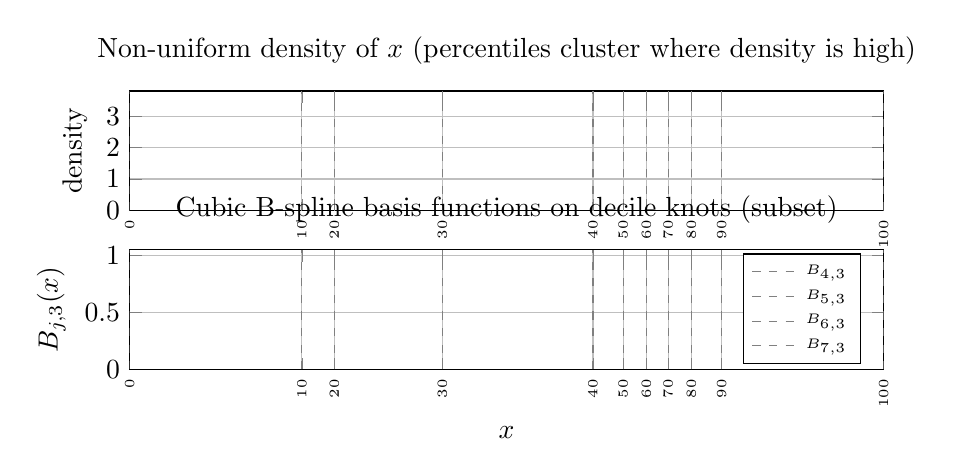
\begin{tikzpicture}
\begin{groupplot}[
  group style={group size=1 by 2, vertical sep=5mm},
  width=0.92\textwidth, height=3.1cm,
  xmin=0, xmax=1, grid=major,
  xtick={0.00000,0.22846,0.27153,0.41488,0.61458,0.65471,0.68559,0.71439,0.74526,0.78538,1.00000},
  xticklabels={0,10,20,30,40,50,60,70,80,90,100},
  xticklabel style={font=\tiny, rotate=90, anchor=east},
]
\nextgroupplot[title={Non-uniform density of $x$ (percentiles cluster where density is high)}, ylabel={density}, ymin=0, ymax=3.8]
\addplot[thick, black] coordinates {\NonUniformDensity};
\foreach \k in {0.00000,0.22846,0.27153,0.41488,0.61458,0.65471,0.68559,0.71439,0.74526,0.78538,1.00000} {%
  \addplot[gray, dashed] coordinates {(\k,0) (\k,3.8)};%
}

\nextgroupplot[title={Cubic B-spline basis functions on decile knots (subset)}, xlabel={$x$}, ylabel={$B_{j,3}(x)$}, ymin=0, ymax=1.05, legend pos=north east, legend style={font=\tiny}]
\addplot[thick, blue] coordinates {\CubicBasisA};
\addplot[thick, red] coordinates {\CubicBasisB};
\addplot[thick, green!60!black] coordinates {\CubicBasisC};
\addplot[thick, orange] coordinates {\CubicBasisD};
\legend{$B_{4,3}$,$B_{5,3}$,$B_{6,3}$,$B_{7,3}$}
\foreach \k in {0.00000,0.22846,0.27153,0.41488,0.61458,0.65471,0.68559,0.71439,0.74526,0.78538,1.00000} {%
  \addplot[gray, dashed] coordinates {(\k,0) (\k,1.05)};%
}
\end{groupplot}
\end{tikzpicture}
\end{frame}

% --- Non-uniform knots: impact on recursion weights ---
\begin{frame}{Non-uniform knots change the Cox--de Boor weights}
\small
The recursion coefficients depend on \textbf{knot distances}:
\[
B_{j,d}(x)=
\frac{x-t_j}{t_{j+d}-t_j}B_{j,d-1}(x)
\;+\;
\frac{t_{j+d+1}-x}{t_{j+d+1}-t_{j+1}}B_{j+1,d-1}(x)
\]
\begin{itemize}
    \item If $t_{j+d}-t_j$ is \textbf{small} (dense knots), the weight ramps faster $\Rightarrow$ basis functions change more rapidly in $x$ (more local detail).
    \item If it is \textbf{large} (sparse knots), the weight varies slowly $\Rightarrow$ broader basis functions (more global influence).
    \item Unequal gaps can make basis functions \textbf{skewed} (different left/right slopes), even for the same degree $d$.
\end{itemize}
\textbf{Practical note:} quantile knots are popular because they roughly equalize data per interval, but you still need regularization (e.g.\ a spline penalty) to control smoothness.
\end{frame}

\begin{frame}{What are GAMs?}
\textbf{Generalized Additive Models} extend linear models by letting each predictor enter through a \emph{flexible} function instead of a single coefficient, while keeping effects \textbf{additive}:
\[
g(E[y \mid X]) = \beta_0 + f_1(X_1) + f_2(X_2) + \cdots + f_p(X_p)
\]
\begin{itemize}
    \item $y$ = response; $X_1, \ldots, X_p$ = predictors.
    \item $f_j$ = smooth or structured terms (splines, factors, etc.), not necessarily linear.
    \item $g$ = link function connecting the mean $E[y]$ to the additive predictor $\eta = \beta_0 + \sum_j f_j(X_j)$.
\end{itemize}
\vspace{2mm}
So a GAM is a \textbf{GLM} (distribution + link) with \textbf{additive} predictor where each $f_j$ can be non-linear. We get interpretable, flexible fits and can plot each $f_j$ separately.
\end{frame}

\begin{frame}{Role of the \textbf{Distribution}}
The \textbf{distribution} describes the randomness of the response $y$ (e.g.\ Normal, Binomial, Poisson). It answers: ``What kind of data is $y$?''
\begin{itemize}
    \item \textbf{Normal}: continuous $y$, any sign (wages, temperature, residuals).
    \item \textbf{Binomial}: binary or proportion (default yes/no, success rate).
    \item \textbf{Poisson}: counts or rates (events per day, number of claims).
    \item \textbf{Gamma}: positive continuous (durations, sizes, amounts $> 0$).
\end{itemize}
Choosing the right distribution fixes the likelihood and the scale of $E[y]$ (e.g.\ counts stay non-negative). In pyGAM you pick a \textbf{class} (e.g.\ \texttt{LinearGAM}, \texttt{PoissonGAM}) that implies the distribution.
\end{frame}

\begin{frame}{Roles of the \textbf{Link} and \textbf{Functional form}}
\textbf{Link function $g$}: connects the mean $\mu = E[y]$ to the linear predictor $\eta = \beta_0 + \sum_j f_j(X_j)$ via $\eta = g(\mu)$, so $\mu = g^{-1}(\eta)$. It ensures the model respects the scale of $y$ (e.g.\ $\mu > 0$ for counts).
\begin{itemize}
    \item \textbf{Identity}: $\eta = \mu$ (continuous $y$, any sign).
    \item \textbf{Logit}: $\eta = \log\frac{p}{1-p}$ (probabilities in $(0,1)$).
    \item \textbf{Log}: $\eta = \log\mu$ (counts, rates, positive means).
\end{itemize}
\vspace{1mm}
\textbf{Functional form}: how each predictor enters the sum (linear $l()$, smooth $s()$, factor $f()$, interaction $te()$). It controls flexibility and interpretability of each term.
\end{frame}

\begin{frame}{Tensor-product terms \texttt{te()}: what 2D functions are allowed?}
\small
A tensor-product term models a \textbf{2D smooth surface}:
\[
f(x,z)\ \approx\ \sum_{k=1}^{K_x}\sum_{\ell=1}^{K_z} c_{k\ell}\, B_k(x)\, C_\ell(z)
\]
where $\{B_k\}$ and $\{C_\ell\}$ are 1D spline bases on $x$ and $z$ (often cubic B-splines).

\begin{itemize}
    \item \textbf{Allowed 2D functions}: any \emph{sufficiently smooth} surface on the domain can be approximated by increasing $(K_x,K_z)$. The surface is \textbf{continuous} and has smooth derivatives (depending on spline degree and knot repetition).
    \item \textbf{Interaction structure}: this is a true interaction term (not additive): it captures patterns that cannot be written as $f_1(x)+f_2(z)$.
    \item \textbf{Anisotropy is allowed}: you can have different complexity/smoothness in each direction (e.g.\ wiggly in $x$, smooth in $z$) by using different basis sizes and/or separate penalties.
    \item \textbf{What it does \emph{not} allow cheaply}: sharp discontinuities or very localized ``corners'' require many knots/basis functions; without them the smoothness penalty will smear such features.
\end{itemize}
\vspace{1mm}
\textbf{In pyGAM}: \texttt{te(0,1)} builds such a tensor-product spline surface in features 0 and 1 (with regularization controlling smoothness).
\end{frame}

\begin{frame}{Functional form in more detail}
The \textbf{functional form} says how each $f_j(X_j)$ is built. In pyGAM you specify it term-by-term:
\begin{itemize}
    \item \textbf{$l(j)$} (linear): $f_j(X_j) = \beta_j X_j$. Straight line; use when the effect is plausibly linear.
    \item \textbf{$s(j)$} (spline): $f_j$ is a smooth curve (e.g.\ P-spline). Use for continuous predictors when you want to capture non-linear effects without choosing knots by hand.
    \item \textbf{$f(j)$} (factor): $f_j$ is a different level per category (e.g.\ one coefficient per education level). Use for categorical predictors.
    \item \textbf{$te(j,k)$} (tensor product): smooth interaction in $X_j$ and $X_k$ (a 2D surface). Use when the effect of one predictor depends on the value of another.
\end{itemize}
Example: \texttt{s(0) + s(1) + f(2)} = smooth in feature 0, smooth in feature 1, factor in feature 2; all effects add on the link scale.
\end{frame}

\begin{frame}{Three building blocks}
Every GAM is: \textbf{Distribution} + \textbf{Link} + \textbf{Functional form}
\[
g(E[y\mid X]) = \beta_0 + f_1(X_1) + f_2(X_2) + \cdots
\]
\begin{center}
\small
\begin{tabular}{lll}
\toprule
\textbf{Distribution} & \textbf{Link $g$} & \textbf{Response type} \\
\midrule
Normal & identity & Continuous (any sign) \\
Binomial & logit & Binary / proportions \\
Poisson & log & Counts ($\ge 0$) \\
Gamma & log & Positive continuous \\
\bottomrule
\end{tabular}
\end{center}
\begin{itemize}
    \item Choose \textbf{distribution} from data type (count, binary, continuous).
    \item \textbf{Link} maps mean to linear predictor (log ensures $\lambda>0$, logit ensures $p\in(0,1)$).
    \item \textbf{Functional form}: how each predictor enters ($l$, $s$, $f$, $te$).
\end{itemize}
\end{frame}

\begin{frame}{Distribution + link: quick reference}
\begin{center}
\small
\begin{tabular}{llll}
\toprule
\textbf{pyGAM class} & \textbf{Distribution} & \textbf{Link} & \textbf{Typical use} \\
\midrule
\texttt{LinearGAM} & Normal & identity & Regression, continuous $y$ \\
\texttt{LogisticGAM} & Binomial & logit & Classification, binary $y$ \\
\texttt{PoissonGAM} & Poisson & log & Counts, rates, event data \\
\texttt{GammaGAM} & Gamma & log & Positive continuous, sizes \\
\texttt{GAM(...)} & custom & custom & e.g.\ \texttt{gamma} + \texttt{log} \\
\bottomrule
\end{tabular}
\end{center}
\end{frame}

% ---------- LinearGAM ----------
\begin{frame}[fragile]{Example 1: Normal + identity (LinearGAM)}
\small
\textbf{Data}: continuous $y$ (e.g.\ wage, acceleration). \textbf{Model}: $E[y] = \beta_0 + f_1(x_1) + f_2(x_2)$ (identity link).
\begin{lstlisting}
# Import the GAM class + the term constructors
from pygam import LinearGAM, s, f
# Load a built-in demo dataset (wage regression)
from pygam.datasets import wage
import matplotlib.pyplot as plt  # plotting

# X: features, y: response (continuous wage)
X, y = wage()
# X columns: [year, age, education]

# Build the additive model: smooth(year) + smooth(age) + factor(education)
gam = LinearGAM(s(0) + s(1) + f(2))
# Fit + tune smoothing strength (lambda) via cross-validated grid search
gam.gridsearch(X, y)

# Partial dependence for term=0 (the smooth of year)
XX = gam.generate_X_grid(term=0)  # grid over year; other features held fixed
pdep, ci = gam.partial_dependence(term=0, X=XX, width=0.95)  # pointwise CI: pdep +/- 1.96*SE

# Plot the estimated effect of year on the response scale
plt.plot(XX[:, 0], pdep, label="effect")
plt.fill_between(XX[:, 0], ci[:, 0], ci[:, 1], alpha=0.3, label="95% CI")
plt.legend()
\end{lstlisting}
\end{frame}

\begin{frame}[fragile]{Example 1: visualize dependence on \emph{all} variables}
\small
To visualize the learned dependence for \textbf{each term}, loop over terms and plot their partial dependence on separate axes.

\begin{lstlisting}
fig, axes = plt.subplots(1, 3, figsize=(11, 3), constrained_layout=True)

for term, ax in enumerate(axes):
    XX = gam.generate_X_grid(term=term)  # varies only the term's feature(s)
    pdep, ci = gam.partial_dependence(term=term, X=XX, width=0.95)

    if term in (0, 1):  # smooth terms: year, age
        x = XX[:, term]              # x values for this term
        ax.plot(x, pdep, lw=2)       # line: estimated effect f(x)
        ax.fill_between(x, ci[:,0], ci[:,1], alpha=0.25)  # shaded CI band
    else:               # factor term: education (categorical)
        levels = XX[:, 2]            # unique category codes/levels
        ax.bar(levels, pdep, alpha=0.7)  # bars: effect per level

    ax.set_title(f"term {term}")
    ax.axhline(0, color="k", lw=0.8, alpha=0.3)  # reference baseline
\end{lstlisting}
\end{frame}

\begin{frame}{Example 1: what the visualization commands do}
\small
\begin{itemize}
    \item \textbf{\texttt{plt.subplots(1,3,...)}}: create a row of axes (one per term) so you can compare effects side-by-side.
    \item \textbf{\texttt{generate\_X\_grid(term=i)}}: creates a grid of $X$ values where \emph{only} the $i$-th term varies (others held fixed).
    \item \textbf{\texttt{partial\_dependence(term=i, X=XX)}}: returns the term contribution $\hat f_i(x)$ (and CI) evaluated on that grid.
    \item \textbf{\texttt{ax.plot(x, pdep)}}: draws the estimated smooth effect as a curve.
    \item \textbf{\texttt{ax.fill\_between(x, low, high)}}: shades the CI band between lower/upper curves.
    \item \textbf{\texttt{ax.bar(levels, pdep)}}: for a factor term, show the effect at each category level.
\end{itemize}
\end{frame}

\begin{frame}{Example 1: partial dependence for all terms (schematic)}
\centering
\small LinearGAM on wage: $s(\mathrm{year}) + s(\mathrm{age}) + f(\mathrm{education})$.
\vspace{1mm}
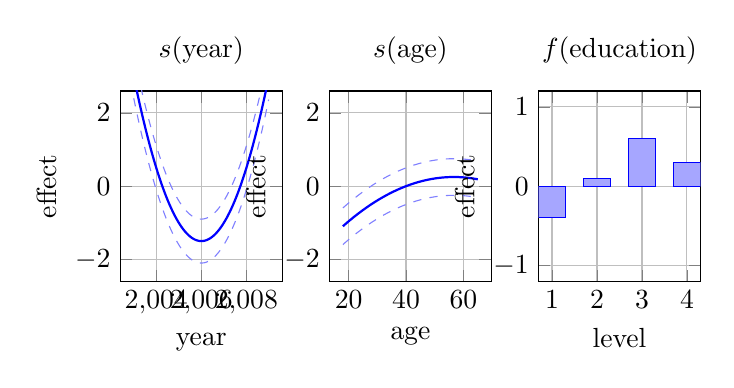
\begin{tikzpicture}
\begin{groupplot}[
  group style={group size=3 by 1, horizontal sep=6mm},
  width=0.30\textwidth, height=4.0cm,
  grid=major, ymin=-2.6, ymax=2.6,
]
\nextgroupplot[title={$s(\mathrm{year})$}, xlabel={year}, ylabel={effect}]
\addplot[thick, blue, domain=2003:2009, samples=80] {0.5*(x-2006)^2 - 1.5};
\addplot[thin, blue!50, dashed, domain=2003:2009, samples=80] {0.5*(x-2006)^2 - 0.9};
\addplot[thin, blue!50, dashed, domain=2003:2009, samples=80] {0.5*(x-2006)^2 - 2.1};

\nextgroupplot[title={$s(\mathrm{age})$}, xlabel={age}, ylabel={effect}]
\addplot[thick, blue, domain=18:65, samples=80] {0.03*(x-40) - 0.0009*(x-40)^2};
\addplot[thin, blue!50, dashed, domain=18:65, samples=80] {0.03*(x-40) - 0.0009*(x-40)^2 + 0.5};
\addplot[thin, blue!50, dashed, domain=18:65, samples=80] {0.03*(x-40) - 0.0009*(x-40)^2 - 0.5};

\nextgroupplot[title={$f(\mathrm{education})$}, xlabel={level}, ylabel={effect}, ymin=-1.2, ymax=1.2]
\addplot[ybar, fill=blue!35, draw=blue] coordinates {(1,-0.4) (2,0.1) (3,0.6) (4,0.3)};
\end{groupplot}
\end{tikzpicture}
\end{frame}

\begin{frame}{Example 1: LinearGAM — partial dependence figure}
\centering
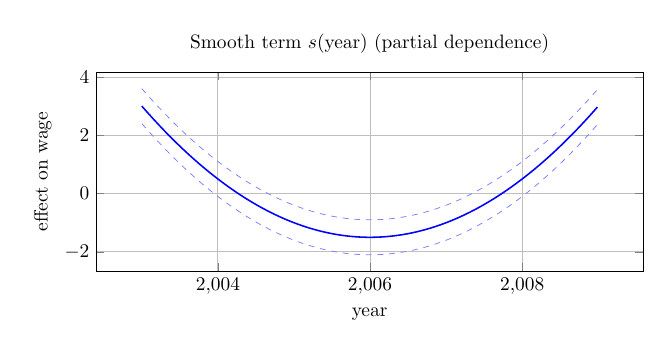
\begin{tikzpicture}[scale=0.7]
\begin{axis}[width=11.5cm, height=5.2cm,
  xlabel={year}, ylabel={effect on wage},
  title={Smooth term $s(\mathrm{year})$ (partial dependence)},
  grid=major, xtick={2004,2006,2008}]
\addplot[thick, blue, domain=2003:2009, samples=80]
  {0.5*(x-2006)^2 - 1.5};
\addplot[thin, blue!50, dashed, domain=2003:2009, samples=80]
  {0.5*(x-2006)^2 - 1.5 + 0.6};
\addplot[thin, blue!50, dashed, domain=2003:2009, samples=80]
  {0.5*(x-2006)^2 - 1.5 - 0.6};
\end{axis}
\end{tikzpicture}
\vspace{1mm}
\small Smooth $s(\mathrm{year})$: non-linear trend (partial dependence) with a schematic 95\% CI.

\vspace{1mm}
\scriptsize
In pyGAM this CI is typically \textbf{pointwise}: $\hat f(x)\pm z_{0.975}\,\mathrm{SE}\{\hat f(x)\}$, where $\mathrm{SE}$ comes from the (penalized) coefficient covariance.
\end{frame}

\begin{frame}{Example 1: LinearGAM — what you see}
\begin{itemize}
    \item \textbf{Distribution}: Normal (continuous outcome).
    \item \textbf{Link}: identity $\Rightarrow$ $E[y] = \eta$ (linear predictor can be any real).
    \item \textbf{Terms}: $s(0)$, $s(1)$ = smooth (spline) effects; $f(2)$ = factor (categorical) effect.
    \item Plot: partial dependence of one term (e.g.\ year) on the scale of the response (wage).
\end{itemize}
\end{frame}

% ---------- LogisticGAM ----------
\begin{frame}[fragile]{Example 2: Binomial + logit (LogisticGAM)}
\small
\textbf{Data}: binary $y$ (e.g.\ default yes/no). \textbf{Model}: $\log\frac{P(y=1)}{P(y=0)} = \beta_0 + f_1(x_1) + s(x_2) + s(x_3)$.
\begin{lstlisting}
# Import a classification GAM + term constructors
from pygam import LogisticGAM, f, s
# Demo dataset for default prediction
from pygam.datasets import default
import matplotlib.pyplot as plt

# Return X,y directly (y is binary: 0/1)
X, y = default(return_X_y=True)
# X columns: [student, balance, income]

# Build the model: factor(student) + smooth(balance) + smooth(income)
gam = LogisticGAM(f(0) + s(1) + s(2))
# Fit + tune smoothing (lambda) via grid search / CV
gam.gridsearch(X, y)

# Partial dependence of the balance term (term=1) on the logit (log-odds) scale
XX = gam.generate_X_grid(term=1)  # grid over balance
pdep, ci = gam.partial_dependence(term=1, X=XX, width=0.95)
plt.plot(XX[:, 1], pdep)  # effect on log-odds of default
# (Optional) convert to probability: p = exp(eta) / (1 + exp(eta))
\end{lstlisting}
\end{frame}

\begin{frame}[fragile]{Example 2: visualize dependence on \emph{all} variables}
\small
For LogisticGAM, partial dependence is on the \textbf{logit (log-odds) scale}. Plot each term to see what drives risk.

\begin{lstlisting}
fig, axes = plt.subplots(1, 3, figsize=(11, 3), constrained_layout=True)

for term, ax in enumerate(axes):
    XX = gam.generate_X_grid(term=term)
    pdep, ci = gam.partial_dependence(term=term, X=XX, width=0.95)

    if term == 0:  # factor: student
        levels = XX[:, 0]
        ax.bar(levels, pdep, alpha=0.7)
    else:          # smooth: balance or income
        x = XX[:, term]
        ax.plot(x, pdep, lw=2)
        ax.fill_between(x, ci[:,0], ci[:,1], alpha=0.25)

    ax.set_title(f"term {term}")
    ax.axhline(0, color="k", lw=0.8, alpha=0.3)
\end{lstlisting}
\end{frame}

\begin{frame}{Example 2: partial dependence for all terms (schematic)}
\centering
\small LogisticGAM: $f(\mathrm{student}) + s(\mathrm{balance}) + s(\mathrm{income})$ (effects on log-odds).
\vspace{1mm}
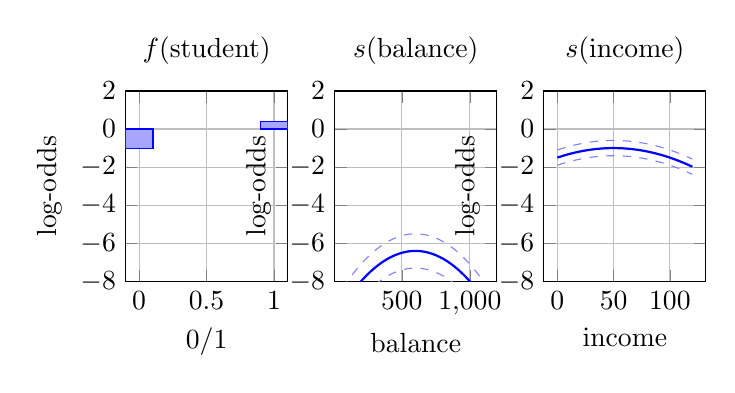
\begin{tikzpicture}
\begin{groupplot}[
  group style={group size=3 by 1, horizontal sep=6mm},
  width=0.30\textwidth, height=4.0cm,
  grid=major, ymin=-8, ymax=2,
]
\nextgroupplot[title={$f(\mathrm{student})$}, xlabel={0/1}, ylabel={log-odds}]
\addplot[ybar, fill=blue!35, draw=blue] coordinates {(0,-1.0) (1,0.4)};

\nextgroupplot[title={$s(\mathrm{balance})$}, xlabel={balance}, ylabel={log-odds}]
\addplot[thick, blue, domain=0:2650, samples=100] {-10 + 0.012*x - 1e-5*x^2};
\addplot[thin, blue!50, dashed, domain=0:2650, samples=100] {-10 + 0.012*x - 1e-5*x^2 + 0.9};
\addplot[thin, blue!50, dashed, domain=0:2650, samples=100] {-10 + 0.012*x - 1e-5*x^2 - 0.9};

\nextgroupplot[title={$s(\mathrm{income})$}, xlabel={income}, ylabel={log-odds}]
\addplot[thick, blue, domain=0:120, samples=100] {-1.5 + 0.02*x - 0.0002*x^2};
\addplot[thin, blue!50, dashed, domain=0:120, samples=100] {-1.5 + 0.02*x - 0.0002*x^2 + 0.4};
\addplot[thin, blue!50, dashed, domain=0:120, samples=100] {-1.5 + 0.02*x - 0.0002*x^2 - 0.4};
\end{groupplot}
\end{tikzpicture}
\end{frame}

\begin{frame}{Example 2: LogisticGAM — partial dependence figure}
\centering
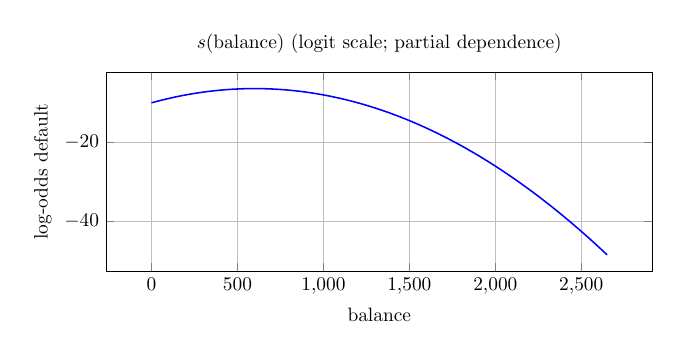
\begin{tikzpicture}[scale=0.7]
\begin{axis}[width=11.5cm, height=5.2cm,
  xlabel={balance}, ylabel={log-odds default},
  title={$s(\mathrm{balance})$ (logit scale; partial dependence)},
  grid=major]
\addplot[thick, blue, domain=0:2650, samples=100]
  {-10 + 0.012*x - 1e-5*x^2};
\end{axis}
\end{tikzpicture}
\vspace{1mm}
\small Higher balance $\Rightarrow$ lower log-odds of default (smooth effect; schematic).
\end{frame}

\begin{frame}{Example 2: LogisticGAM — what you see}
\begin{itemize}
    \item \textbf{Distribution}: Binomial (binary outcome).
    \item \textbf{Link}: logit $\Rightarrow$ linear predictor = log-odds; inverse link gives probability in $(0,1)$.
    \item \textbf{Terms}: $f(0)$ = factor (e.g.\ student yes/no); $s(1)$, $s(2)$ = smooth effects (balance, income).
    \item Partial dependence on log-odds scale; transform with $\frac{e^\eta}{1+e^\eta}$ to get probability.
\end{itemize}
\end{frame}

% ---------- PoissonGAM ----------
\begin{frame}[fragile]{Example 3: Poisson + log (PoissonGAM)}
\small
\textbf{Data}: counts $y$ (e.g.\ events per time bin). \textbf{Model}: $\log E[y] = \beta_0 + f(t)$ $\Rightarrow$ $E[y] = e^{\beta_0 + f(t)}$.
\begin{lstlisting}
# Import a Poisson GAM (for counts) + spline term constructor
from pygam import PoissonGAM, s
import matplotlib.pyplot as plt

# Example data placeholders:
# hour_bins: array of hour indices, counts_per_bin: observed ride counts
X = hour_bins.reshape(-1, 1)  # pyGAM expects 2D X: (n_samples, n_features)
y = counts_per_bin            # counts >= 0

# Model: log E[y] = beta0 + smooth(hour)
gam = PoissonGAM(s(0))
# Fit + tune smoothing strength via grid search / CV
gam.gridsearch(X, y)

# Fitted intensity lambda(x) = E[y|x] (returned on the response scale)
XX = gam.generate_X_grid(term=0)  # grid over hour
lam = gam.predict(XX)             # predicted mean count per hour-bin

# Plot the fitted curve and the observed binned counts
plt.plot(XX, lam, label="fit")
plt.bar(centers, y, width=0.8, alpha=0.6, label="data")  # centers: bin centers
plt.legend()
\end{lstlisting}
\end{frame}

\begin{frame}{Example 3: PoissonGAM — fitted intensity figure}
\centering
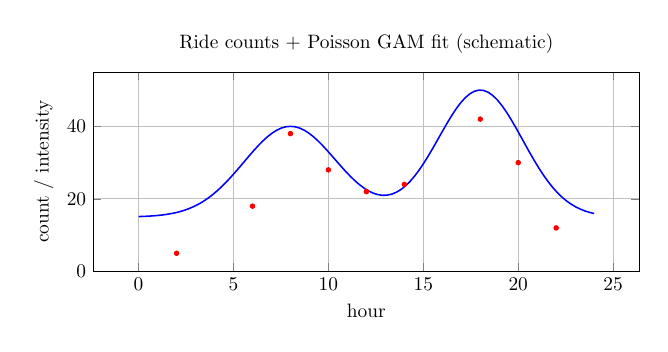
\begin{tikzpicture}[scale=0.7]
\begin{axis}[width=11.5cm, height=5.2cm,
  xlabel={hour}, ylabel={count / intensity},
  title={Ride counts + Poisson GAM fit (schematic)},
  grid=major, ymin=0]
\addplot[thick, blue, domain=0:24, samples=100]
  {15 + 25*exp(-((x-8)^2)/12) 
   + 35*exp(-((x-18)^2)/10)};
\addplot[only marks, mark=*, mark size=1.2pt, red]
  coordinates {(2,5) (6,18) (8,38) (10,28)
   (12,22) (14,24) (18,42) (20,30) (22,12)};
\end{axis}
\end{tikzpicture}
\vspace{1mm}
\small Log link keeps $E[y]>0$; curve = fitted intensity (mean count).
\end{frame}

\begin{frame}{Example 3: PoissonGAM — what you see}
\begin{itemize}
    \item \textbf{Distribution}: Poisson (counts).
    \item \textbf{Link}: log $\Rightarrow$ $\log E[y] = \eta$, so $E[y] = e^\eta > 0$.
    \item \textbf{Terms}: $s(0)$ = smooth effect of time (e.g.\ hour) on rate.
    \item Use for: event counts, rates, time-varying intensity (e.g.\ taxi rides per hour).
\end{itemize}
\end{frame}

% ---------- Functional forms ----------
\begin{frame}{Functional forms: $l()$, $s()$, $f()$, $te()$}
\small
\begin{center}
\begin{tabular}{llp{5.5cm}}
\toprule
\textbf{Term} & \textbf{Meaning} & \textbf{When to use} \\
\midrule
$l(j)$ & Linear & Effect of $x_j$ is $\beta_j x_j$ (straight line). \\
$s(j)$ & Spline (smooth) & Non-linear effect of $x_j$; default in pyGAM. \\
$f(j)$ & Factor & $x_j$ categorical; one coefficient per level. \\
$te(j,k)$ & Tensor product & Interaction: smooth in $x_j$ and $x_k$ together. \\
\bottomrule
\end{tabular}
\end{center}
\vspace{2mm}
Example formula: \texttt{LinearGAM(l(0) + s(1) + f(2) + te(1,3))} \\
$\Rightarrow$ linear in $x_0$, smooth in $x_1$, factor in $x_2$, smooth interaction in $x_1$ and $x_3$.
\end{frame}

\begin{frame}[fragile]{Code: choosing terms}
\begin{lstlisting}
from pygam import LinearGAM, PoissonGAM, l, s, f, te

# Linear only: straight-line effects
gam_linear = LinearGAM(l(0) + l(1)).fit(X, y)  # .fit() trains the model

# Smooth (default for continuous): flexible non-linear effects
gam_smooth = LinearGAM(s(0) + s(1)).fit(X, y)

# Mixed: linear + smooth + factor (categorical)
gam_mixed = LinearGAM(l(0) + s(1) + f(2)).fit(X, y)

# With interaction: tensor-product surface over features 1 and 2
gam_int = PoissonGAM(s(0) + te(1, 2) + s(3)).fit(X, y)
# te(1,2) learns a 2D smooth f(x1, x2) that is not just f1(x1)+f2(x2)
\end{lstlisting}
\end{frame}

\begin{frame}{Partial dependence: one term at a time}
\small
For each term, \texttt{partial\_dependence(term=i)} returns the contribution of that term (on the link scale) over a grid of $x_i$, with other covariates fixed (e.g.\ at means) or marginalized.

\begin{center}
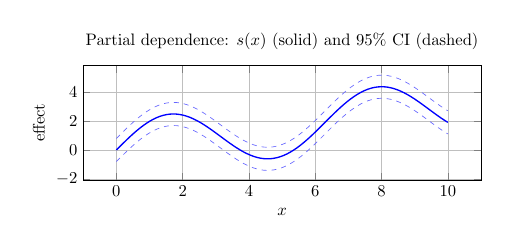
\begin{tikzpicture}[scale=0.6]
\begin{axis}[width=10cm, height=4cm,
  xlabel={$x$}, ylabel={effect},
  title={Partial dependence: $s(x)$ (solid) and 95\% CI (dashed)},
  grid=major]
\addplot[thick, blue, domain=0:10, samples=100] 
  {2*sin(deg(x)) + 0.3*x};
\addplot[thin, blue!60, dashed, domain=0:10, samples=100] 
  {2*sin(deg(x)) + 0.3*x + 0.8};
\addplot[thin, blue!60, dashed, domain=0:10, samples=100] 
  {2*sin(deg(x)) + 0.3*x - 0.8};
\end{axis}
\end{tikzpicture}
\end{center}
Interpretation: “How does the response change as this predictor varies, holding others fixed?”
\end{frame}

\begin{frame}{Summary: pick distribution, link, and terms}
\begin{enumerate}
    \item \textbf{Distribution}: Normal (continuous), Binomial (binary), Poisson (counts), Gamma (positive).
    \item \textbf{Link}: identity (LinearGAM), logit (LogisticGAM), log (PoissonGAM, GammaGAM).
    \item \textbf{Terms}: $l()$ linear, $s()$ smooth, $f()$ factor, $te()$ interaction.
    \item \textbf{Code}: build formula (e.g.\ \texttt{s(0)+f(1)}), \texttt{.gridsearch()} or \texttt{.fit()}, then \texttt{partial\_dependence()} and \texttt{.predict()} for plots and predictions.
\end{enumerate}
\end{frame}

\begin{frame}{References}
\begin{itemize}
    \item pyGAM: \texttt{pygam.readthedocs.io}
    \item Datasets: \texttt{pygam.datasets} (wage, default, mcycle, chicago, coal, trees, etc.)
    \item Hastie \& Tibshirani, \textit{Generalized Additive Models}; Wood, \textit{Generalized Additive Models: An Introduction with R}
\end{itemize}
\end{frame}

\end{document}
